\chapter{Semantics of \aoeexedir{}}
    \label{chp:semantics}
    
    \section{BattleServer}

    Folder with \code{BattleServer.exe} file. Usually not useful when modding.

    \section{certificates}

    \code{X509} file format of \aoe{}. Usually not useful when modding.

    \section{Docs}

    Manual of PDF of \aoe{}. Not useful when modding.

    \section{Schema}

    Not useful when modding.

    \section{Support}

    Contains some link to \aoe{} website support. Not useful when modding.

    \section{Tools\_Builds}

    Represents \genie{} directory.

    \section{webclient}

    Not useful when modding.

    \section{wwise}

    Not useful when modding.

    \section{resources}

    Specifies all the data that are not widgets of the \acrref{UI}. The folder contains data like the cursors icons, the \genie{} dat files.

    \subsection{\_common}

    This is the main folder of \textbf{resources} directory.

    \subsubsection{cursors}

    List of all the cursors the cursor directed by the user mouse will display when a given action is performed. For instance, when you need to garrison a villager, a specific cursor image replace the classic arrow icon. All the cursors image have the \code{cur} extension.

    \subsubsection{dat}

    Contains the dat files containing all the information regarding units, civilization, buildings: \code{empires2\_x2\_p1.dat} contains all such information. \footnote{The file can be opened by \genie{}}

    \subsubsection{drs}

    \paragraph{gamedata\_x2}

    This important folder contains \acrref{RMS} files that can be used in your \acrref{RMS} programming (\eg{} \code{F\_Season.inc}). See Appendix \ref{chp:rms}.

    \section{widgetui}

    Specifies which set of textures \aoe{} needs to display alongside their configuration. If you need to alter a picture, it will probably be here.
    Contains a set of json.
    Furthermore, it contains a folder named \dquote{textures}, representing all the textures and images in the game. There are versions, \textit{textures} and \textit{textures-sd}: the former contains the texture to use and the latter contains the low resolution version of the same textures. The first texture are mandatory while the second are optional (modwise). All textures are saved via \acrref{DDS} extensions.\footnote{You can use \code{Irfan View} 32-bit version to view \acrref{DDS} images.}

    \code{Textures} folder contains other folders:

    \subsection{atlas} 

    Contains textures that are present in the Campaigns menu (\eg{} the scenes where you can choose which campaign to play), Sun Tzu icons in the \dquote{Art of War}, images representing the \acrref{UI} you see while playing (\figref{fig:CivAsia}), the window chat, buildings icons (\figref{fig:ingamebuildings}).

    \begin{figure}
        \centering
        \begin{subfigure}{0.48\textwidth}
            \centering
            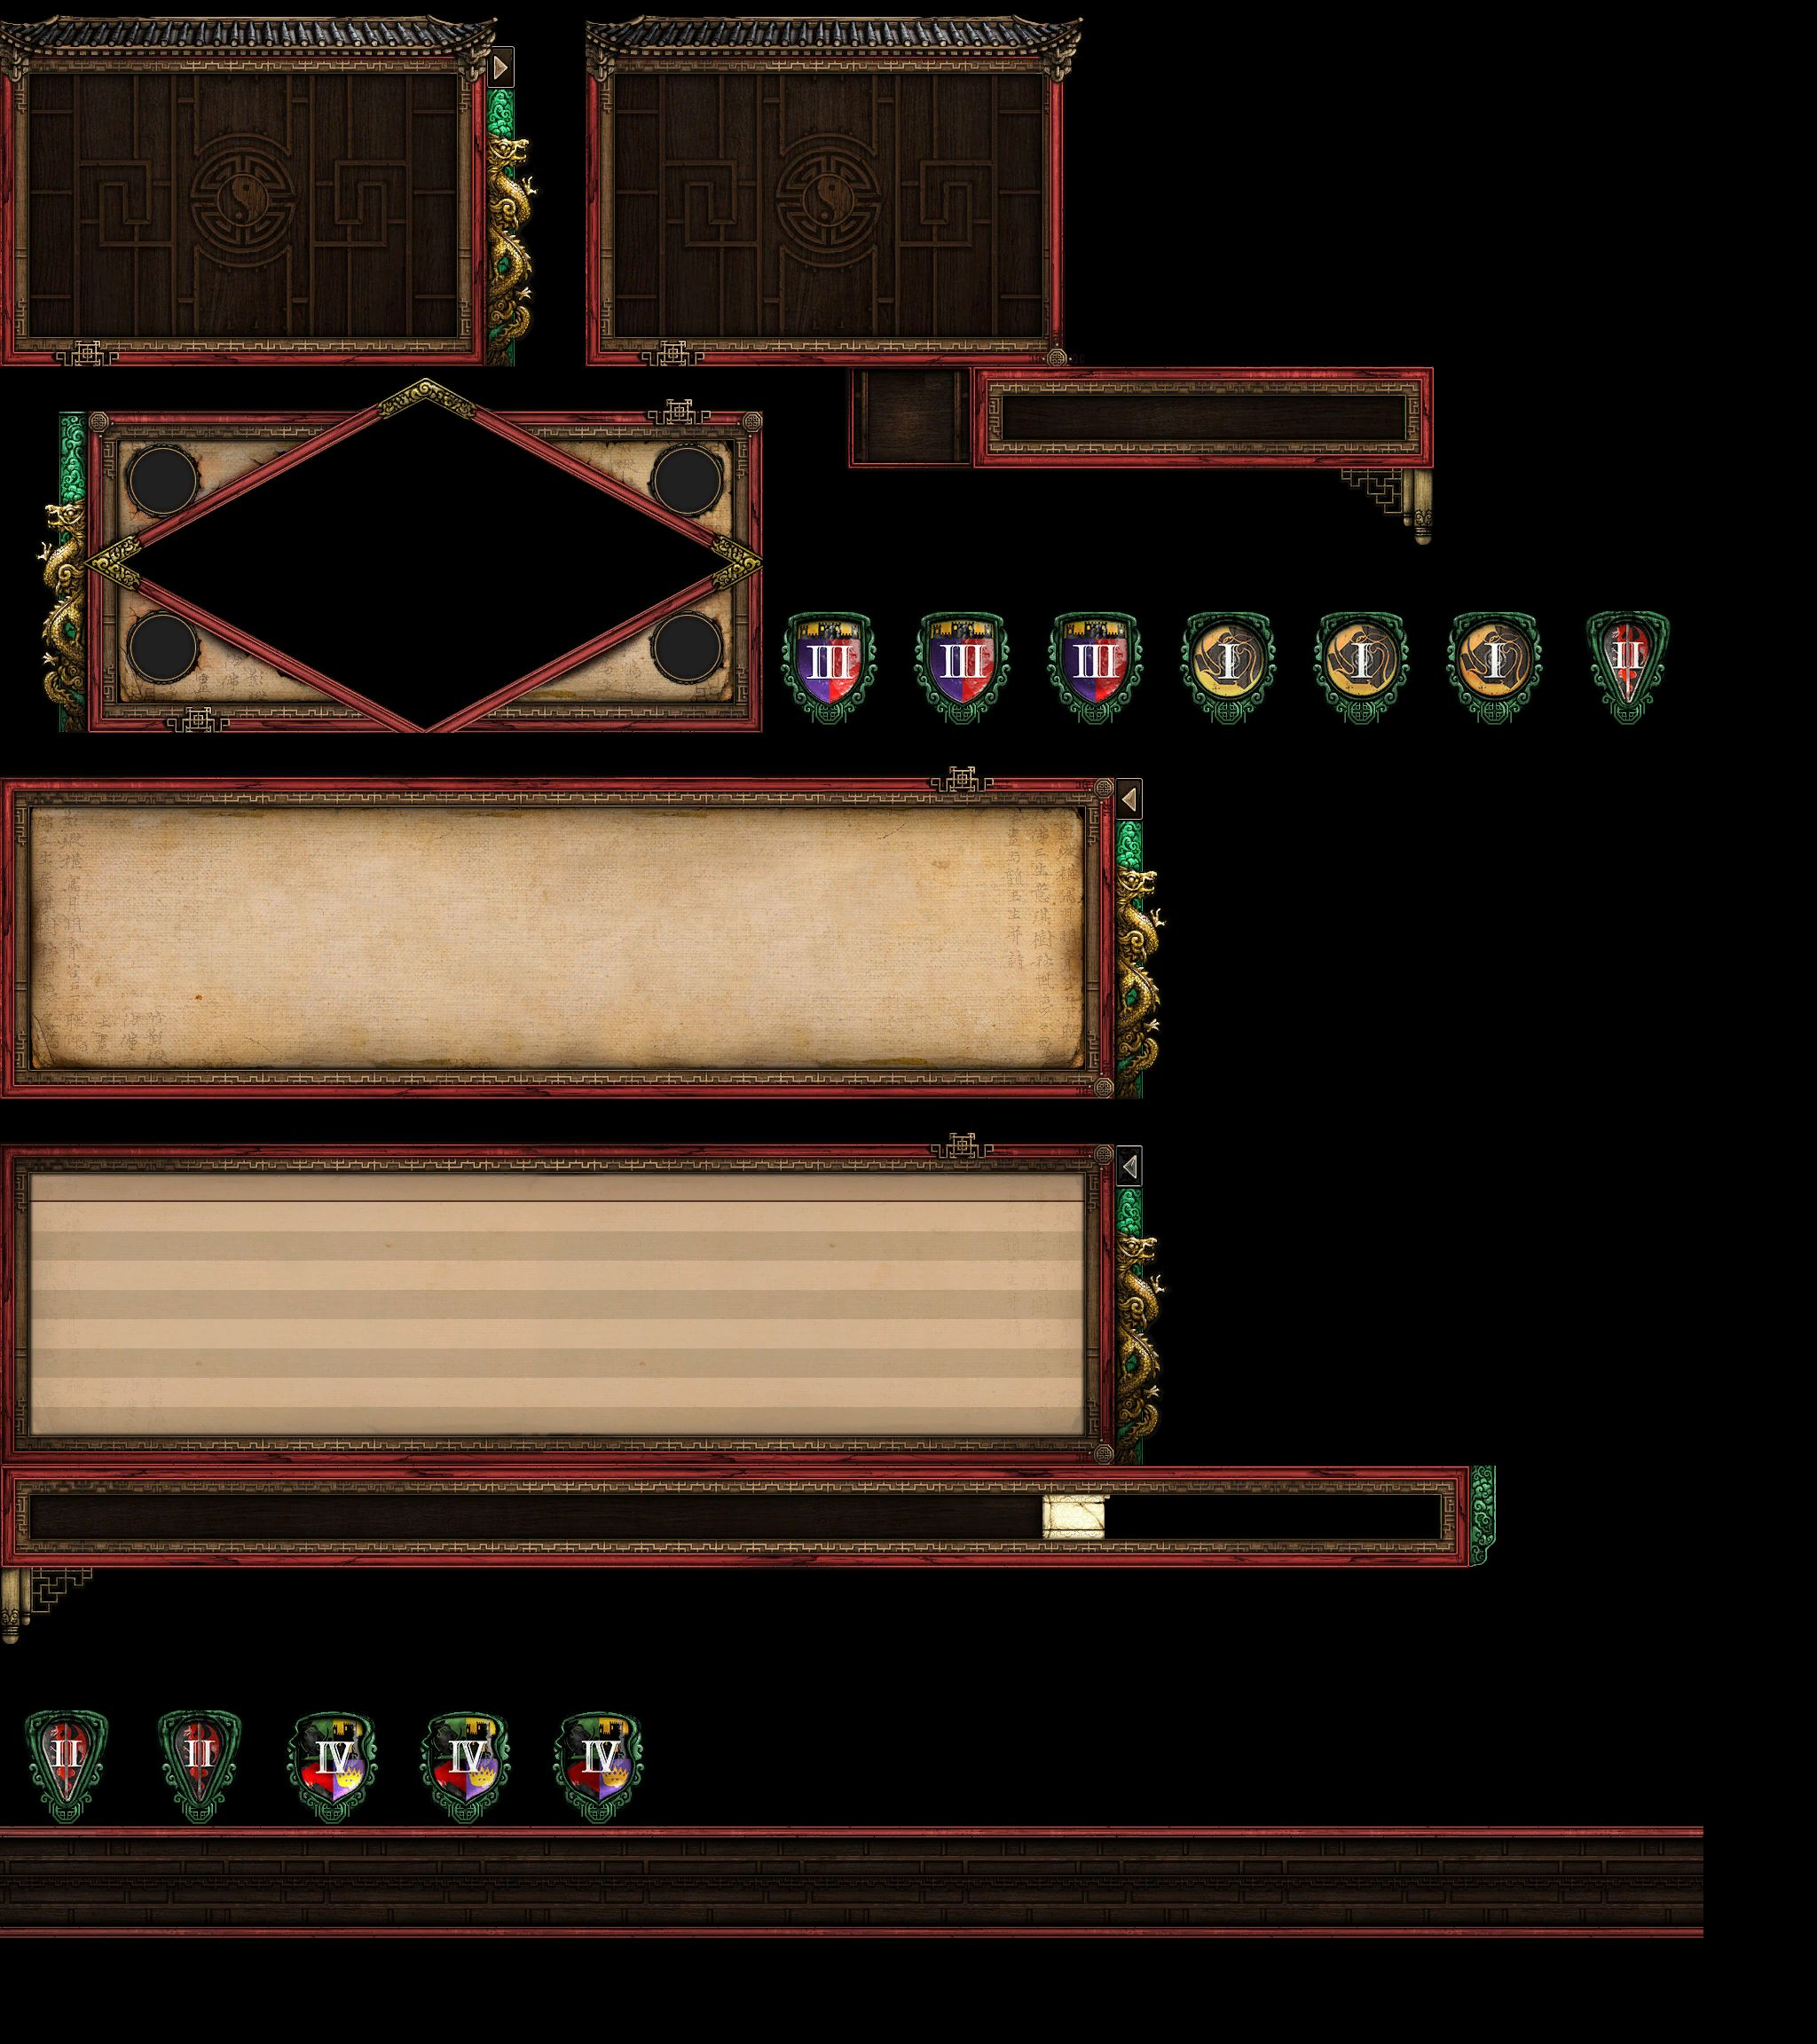
\includegraphics[width=1.0\textwidth]{src/images/CivAsia}
            \caption{CivAsia file, containing the \acrref{UI}}
            \label{fig:CivAsia}
        \end{subfigure}\quad%
        \begin{subfigure}{0.48\textwidth}
            \centering
            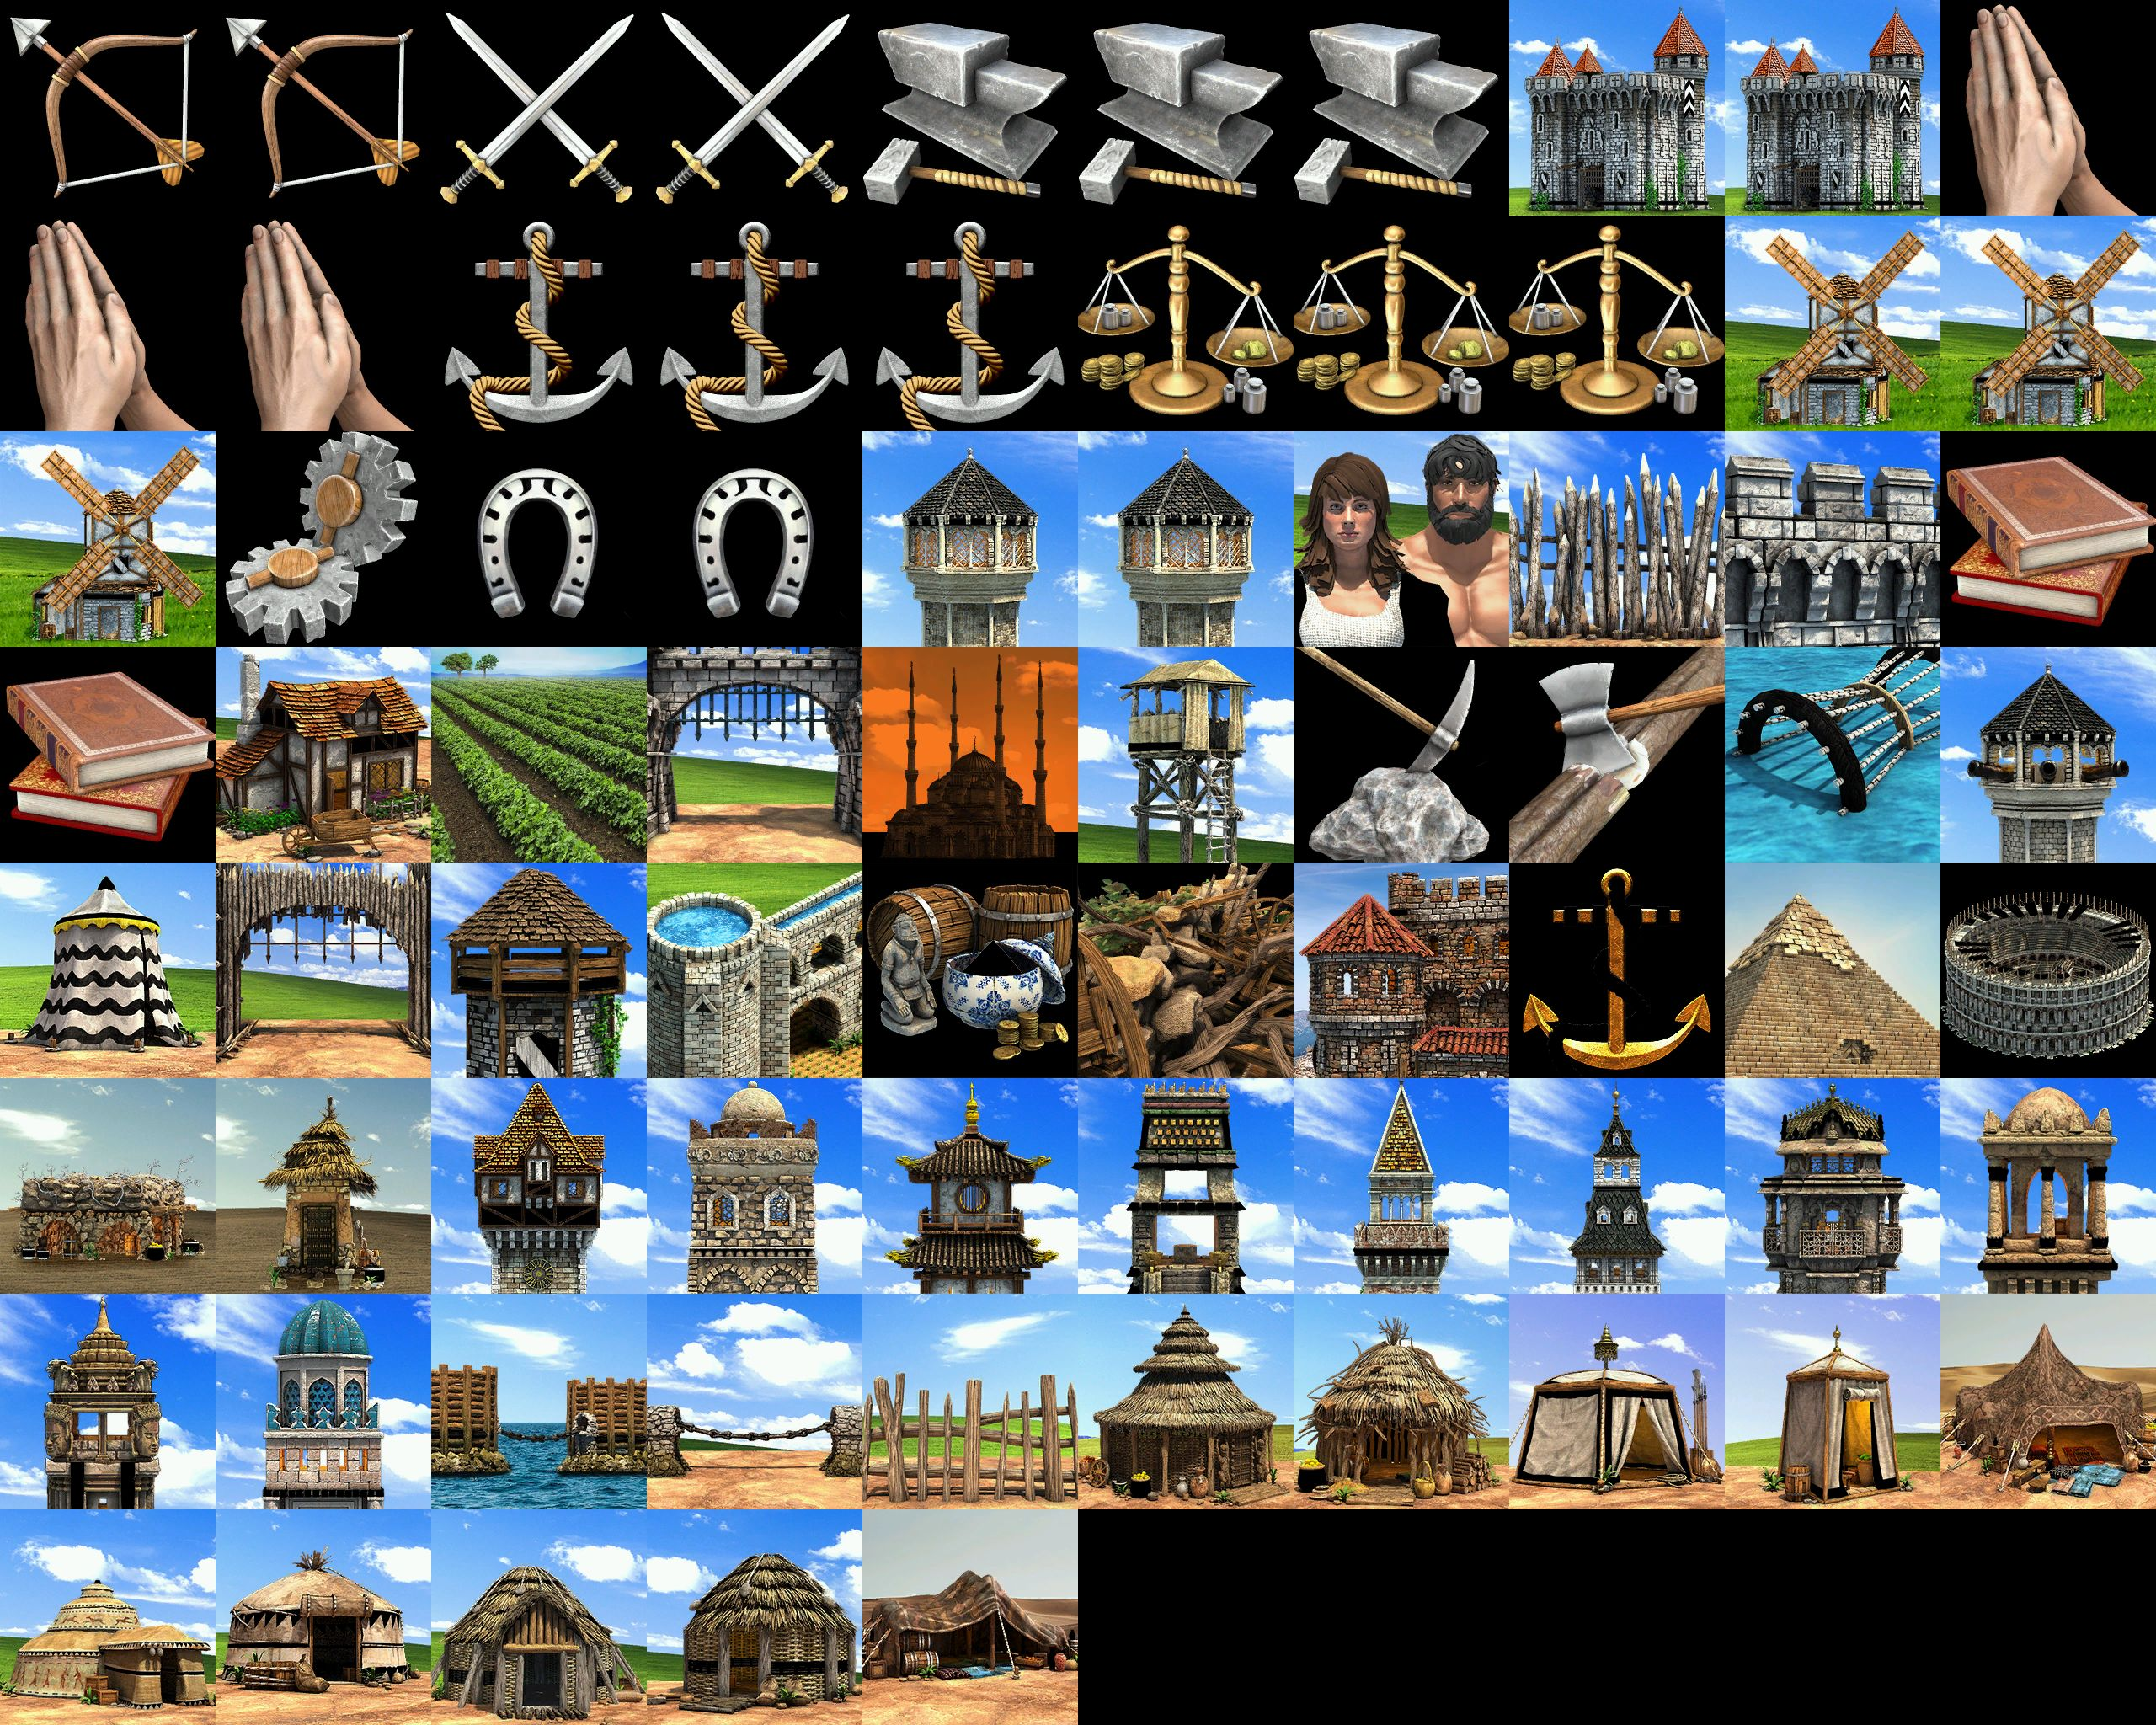
\includegraphics[width=1.0\textwidth]{src/images/ingamebuildings}
            \caption{ingamebuildings file, containing the icons of the buildings in \acrref{UI}}
            \label{fig:ingamebuildings}
        \end{subfigure}\\%
    \end{figure}

    \subsection{backgrounds}

    Contains the menu background (\dquote{mainmenu\_bg} and \dquote{mainmenu\_bg\_1}) images as well the windows in the \aoe{} menus (\eg{} lobby creation, history). Examples of these figures are shown in \figref{fig::backgrounds}. Note that some of images here are represented via \acrref{PNG} rather than \acrref{DDS}.

    \begin{figure}
        \centering
        \begin{subfigure}{0.48\textwidth}
            \centering
            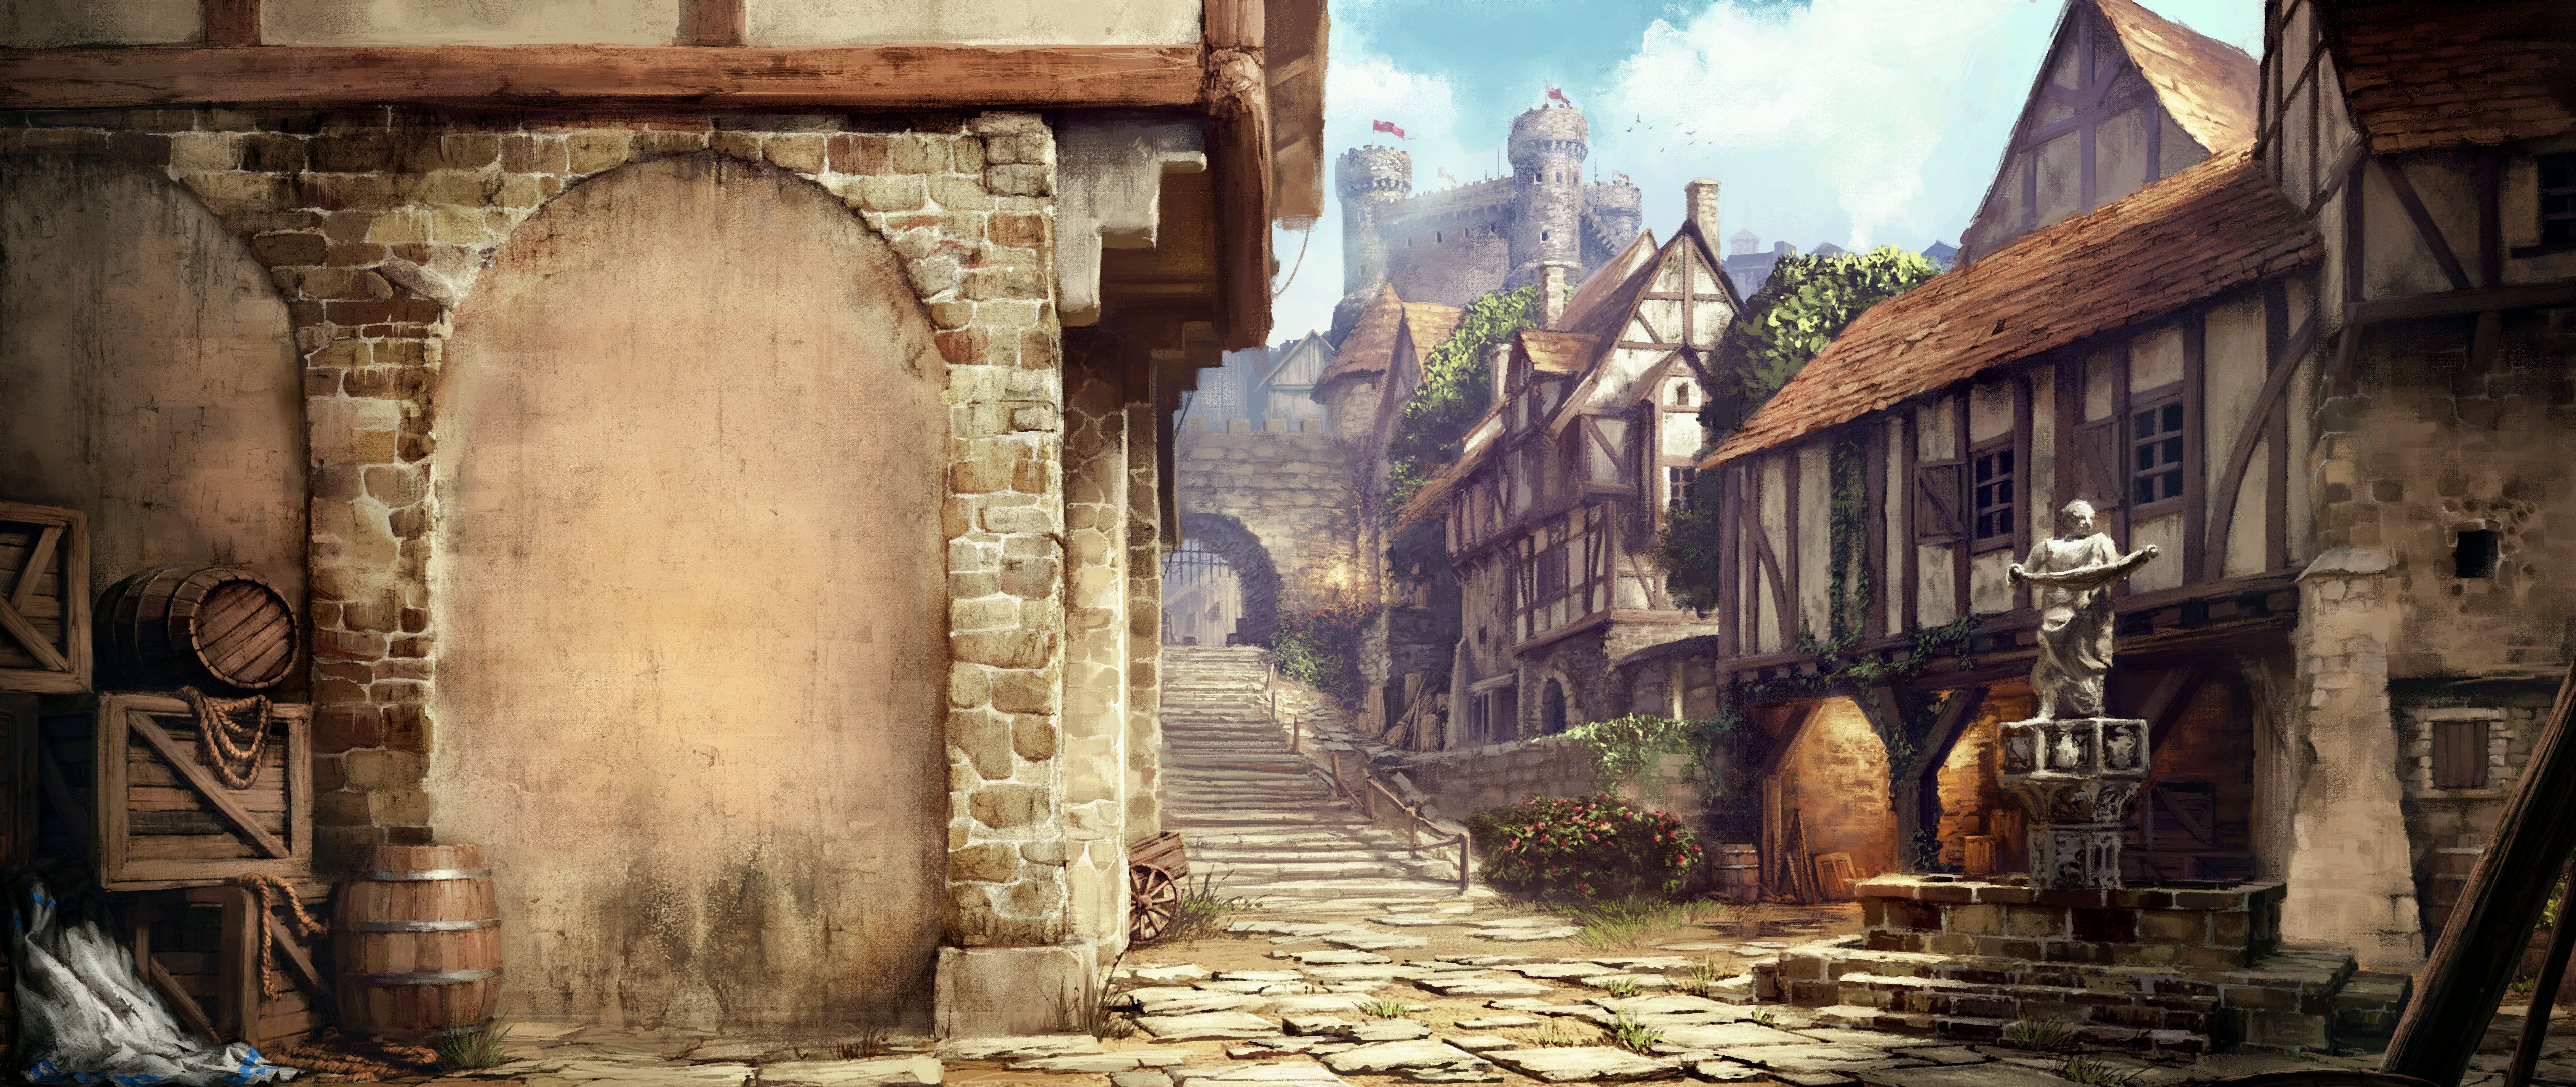
\includegraphics[width=1.0\textwidth]{src/images/mainmenu-bg}
        \end{subfigure}\quad%
        \begin{subfigure}{0.48\textwidth}
            \centering
            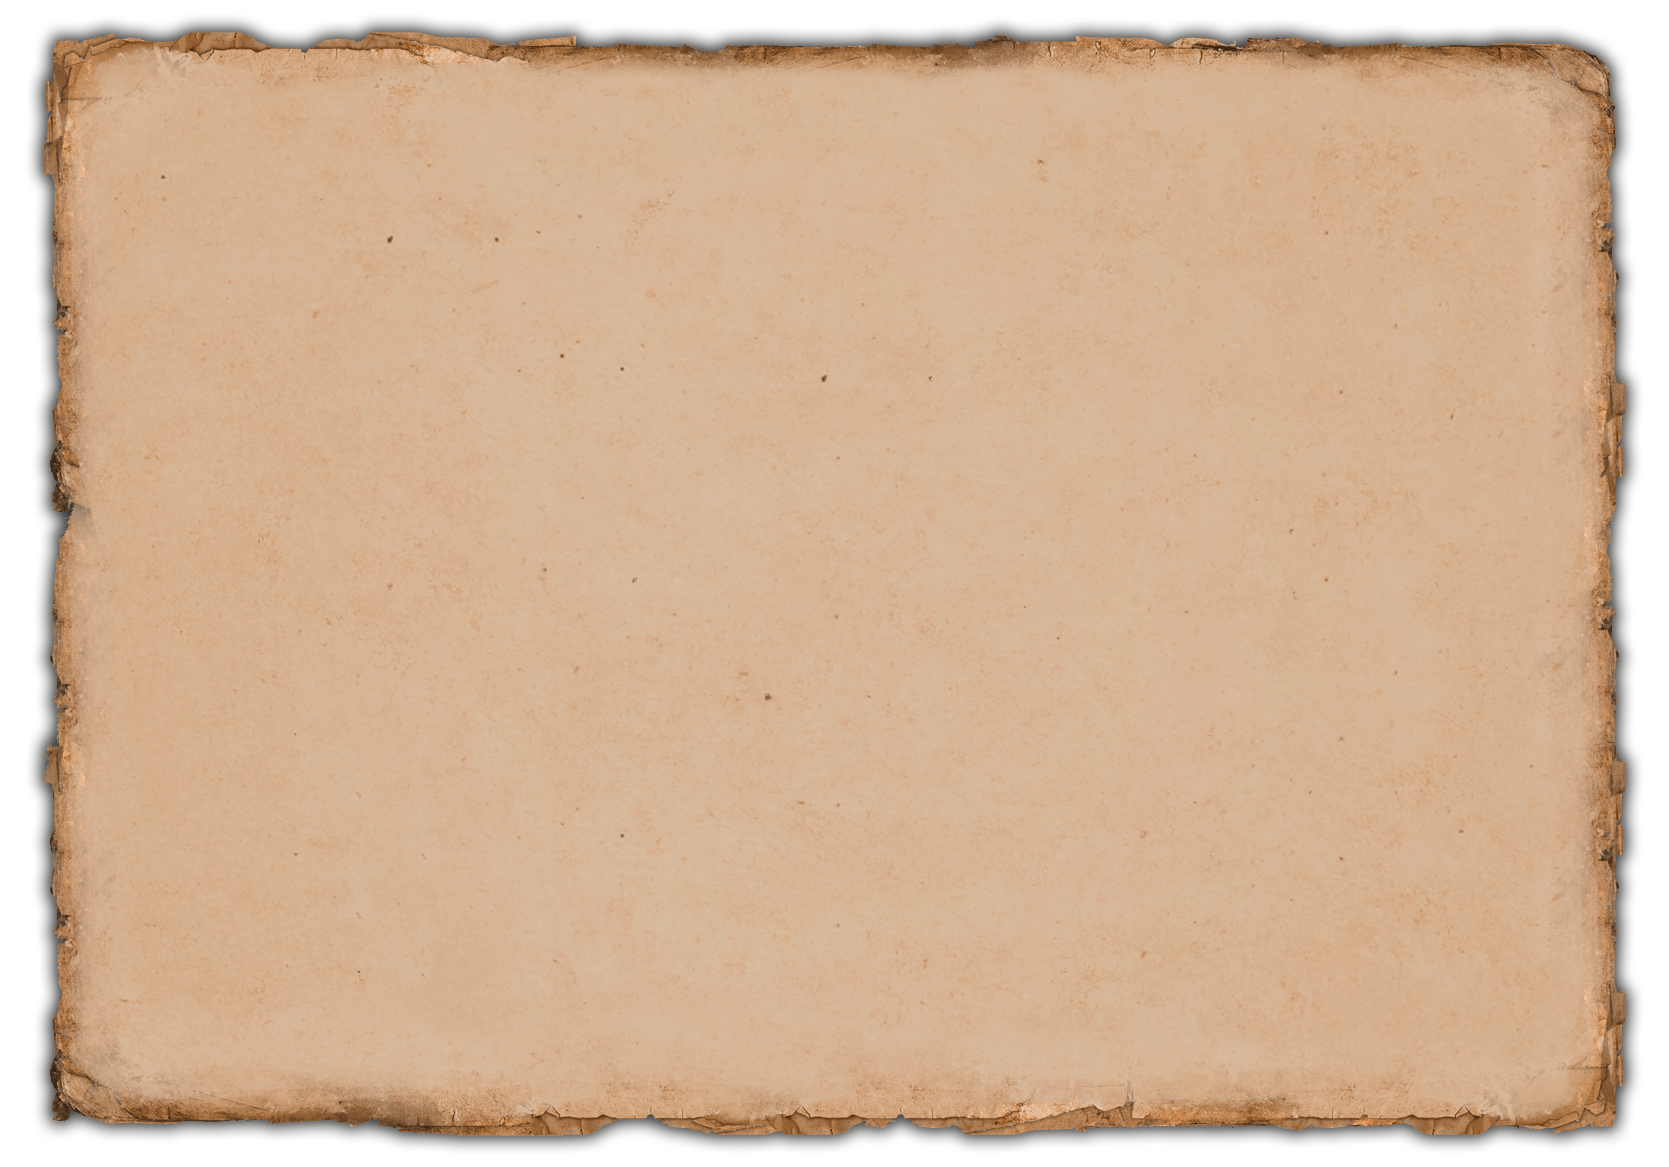
\includegraphics[width=1.0\textwidth]{src/images/popup-menu-bg}
        \end{subfigure}\\%
        \caption{Background menu examples}
        \label{fig:backgrounds}
    \end{figure}

    \subsection{campaign}

    Texture regarding the campaigns, one sub directory per campaign. For instance, \dquote{cam3} is the \textit{Saladin Campaign}. Within it:
    \begin{itemize}
        \item $X.dss$ file, where $X$ is the campaign name, is the campaign image menu file (\ie{} the image where you can choose the specific mission);
        \item $X$\_$background$ is the image where the mission intro and outro are presented;
        \item a subfolder, one per mission in the given campaign. Each sub folder name has a number (starting from 1) as name and contains the drawings in the intro and outros of the associated mission.
    \end{itemize}

    \subsection{ingame}

    TODO

    \subsection{menu}

    TODO